%-------------------------------------------------------------------------------
% Document & Package declarations
%-------------------------------------------------------------------------------

\documentclass[a4paper, 10pt, conference]{ieeeconf}
\usepackage{graphicx}
\usepackage[colorlinks=true, allcolors=black]{hyperref}
\usepackage{tabularx}

%% Language and font encodings
\usepackage[english]{babel}
\usepackage[utf8x]{inputenc}
\usepackage[T1]{fontenc}

%% Useful packages
\usepackage{amsmath}
\usepackage{graphicx}
\usepackage[colorinlistoftodos]{todonotes}
\usepackage[font=footnotesize,labelfont=bf]{caption}
\usepackage[font=footnotesize,labelfont=bf]{subcaption}

%% Packages for displaying source code
\usepackage{listings}
% \usepackage[framed,numbered,autolinebreaks,useliterate]{mcode}

\usepackage{float}
\usepackage{longtable}

%% Packages for displaying source code
\usepackage[numbered,framed]{matlab-prettifier}
\usepackage{color}

%%*************************************************************************
%% Legal Notice:
%% This code is offered as-is without any warranty either expressed or
%% implied; without even the implied warranty of MERCHANTABILITY or
%% FITNESS FOR A PARTICULAR PURPOSE!
%% User assumes all risk.
%% In no event shall IEEE or any contributor to this code be liable for
%% any damages or losses, including, but not limited to, incidental,
%% consequential, or any other damages, resulting from the use or misuse
%% of any information contained here.
%%
%% All comments are the opinions of their respective authors and are not
%% necessarily endorsed by the IEEE.
%%
%% This work is distributed under the LaTeX Project Public License (LPPL)
%% ( http://www.latex-project.org/ ) version 1.3, and may be freely used,
%% distributed and modified. A copy of the LPPL, version 1.3, is included
%% in the base LaTeX documentation of all distributions of LaTeX released
%% 2003/12/01 or later.
%% Retain all contribution notices and credits.
%% ** Modified files should be clearly indicated as such, including  **
%% ** renaming them and changing author support contact information. **
%%
%% File list of work: IEEEtran.cls, IEEEtran_HOWTO.pdf, bare_adv.tex,
%%                    bare_conf.tex, bare_jrnl.tex, bare_jrnl_compsoc.tex,
%%                    bare_jrnl_transmag.tex
%%*************************************************************************

%-------------------------------------------------------------------------------
% Document Configuration
%-------------------------------------------------------------------------------

\begin{document}
\title{Pattern Recognition - Distance Metrics and Neural Networks}
\author{Michael~Hart (00818445) and
        Meng~Kiang~Seah (00699092)
\\
        Department of Electrical and Electronic Engineering,
        Imperial College London,
        SW7 2AZ
\\
        E-mail: \{mh1613, mks211\}@imperial.ac.uk}
\date{\today}

%-------------------------------------------------------------------------------
% Plan on what to write
%-------------------------------------------------------------------------------

% See coursework instructions at:
% https://bb.imperial.ac.uk/bbcswebdav/pid-1009576-dt-content-rid-3417906_1/courses/DSS-EE4_68-16_17/PRCoursework2.pdf

%-------------------------------------------------------------------------------
% Information Banner
%-------------------------------------------------------------------------------

\maketitle

%-------------------------------------------------------------------------------
% Abstract
%-------------------------------------------------------------------------------

\begin{abstract}
\todo{Use actual words} Lorem ipsum dolor sit amet, consectetur adipiscing elit. Vivamus ac faucibus libero, vel facilisis lacus. Cras imperdiet, enim vitae consequat pharetra, dui odio cursus mi, finibus tristique est sapien a dolor. Donec eu dui in elit tempor volutpat id non sapien. Aenean volutpat lectus eu lacinia tincidunt. Donec at libero volutpat, tempus magna ac, gravida est. Integer gravida, ligula id posuere semper, libero justo gravida lorem, non congue odio odio luctus lectus. In hac habitasse platea dictumst. Quisque auctor purus lectus, vitae condimentum libero.
\end{abstract}

%-------------------------------------------------------------------------------
% Introduction
%-------------------------------------------------------------------------------
\section{Introduction}
An introduction to be placed here. Discuss data and partitioning.Lorem ipsum dolor sit amet, consectetur adipiscing elit. Vivamus ac faucibus libero, vel facilisis lacus. Cras imperdiet, enim vitae consequat pharetra, dui odio cursus mi, finibus tristique est sapien a dolor. Donec eu dui in elit tempor volutpat id non sapien. Aenean volutpat lectus eu lacinia tincidunt. Donec at libero volutpat, tempus magna ac, gravida est.
\subsection{Nearest Neighbour Classification}
Lorem ipsum dolor sit amet, consectetur adipiscing elit. Vivamus ac faucibus libero, vel facilisis lacus. Cras imperdiet, enim vitae consequat pharetra, dui odio cursus mi, finibus tristique est sapien a dolor.
\subsection{K-Means Clustering and Classification}
Lorem ipsum dolor sit amet, consectetur adipiscing elit. Vivamus ac faucibus libero, vel facilisis lacus. Cras imperdiet, enim vitae consequat pharetra, dui odio cursus mi, finibus tristique est sapien a dolor. Donec eu dui in elit tempor volutpat id non sapien. Aenean volutpat lectus eu lacinia tincidunt. Donec at libero volutpat, tempus magna ac, gravida est.
\subsection{Neural Networks}
Lorem ipsum dolor sit amet, consectetur adipiscing elit. Vivamus ac faucibus libero, vel facilisis lacus. Cras imperdiet, enim vitae consequat pharetra, dui odio cursus mi, finibus tristique est sapien a dolor. Donec eu dui in elit tempor volutpat id non sapien. Aenean volutpat lectus eu lacinia tincidunt. Donec at libero volutpat, tempus magna ac, gravida est.

%-------------------------------------------------------------------------------
% Distance Metrics
%-------------------------------------------------------------------------------
\section{Distance Metrics}
\subsection{Data Preparation}
The data given can be analysed in its raw form, but it can also be L2-normalised. This means that it is divided by its L2-distance. This is defined as in Equation \ref{eq:l2}, for a $p$-dimensional vector.
\begin{align}
  L_2 &= \sum_{i = 1}^{p} \left( x_i \right) ^2 \label{eq:l2}
\end{align}
The question then becomes whether to normalise all 178 instances by instance (per row) or by dimension (by column). If one were to visualise the data, normalising it by instance would place all points at a Euclidean distance of 1 from the origin. This would mean they would form a hypersphere. In contrast, normalising by dimension places shrinks the spread of the data so that every value fits in the range $[-1; 1]$. From the same source as was used with the Support Vector Machines (SVMs) \cite{scale}, the sensible thing is to normalise by dimension. This prevents any one dimension from becoming overbearing in future measurements. Additionally, it makes no sense to scale the data in one instance with itself, as this will still allow the dimensions with larger variance to dominate.

\subsection{Covariances}
From the unmodified data and the normalised data, the covariances can be calculated, simply by using the full set of data, or by focusing on each of the three class individually. Thus, for the two types of data, there are 4 covariance matrices: all the data, class 1, class 2, and class 3. The way used to obtain the covariance matrices was the \texttt{cov} built-in function in MATLAB.

For context, the way to interpret the data in a covariance matrix is to know that it will be a square, symmetric matrix, with dimensions equal to the number of dimensions in each data instance. The matrix, $S$, will have elements $s_{i, j}$, equal to covariance of the $i$-th and $j$-th dimension. The primary diagonal is the covariance of a dimension with itself, and is therefore the variance \cite{cov}.

Analysing 13 by 13 tables of numbers is not easy. Therefore, a useful alternative is to view the matrices as colour maps, which are easily produced with MATLAB. \todo{INCLUDE IN APPENDIX}

\subsubsection{Unmodifed Training Data}
Figure \ref{fig:covtrainingone} shows the color map for the covariance of the training matrix. The other 3 are found in Appendix \ref{sec:covtraining}, to conserve space. However, they are all like Figure \ref{fig:covtrainingone}. By not performing any scaling to the data, the dimension with the largest range, 13, has dominated the diagram.

\begin{figure}[!ht]
    \centering
    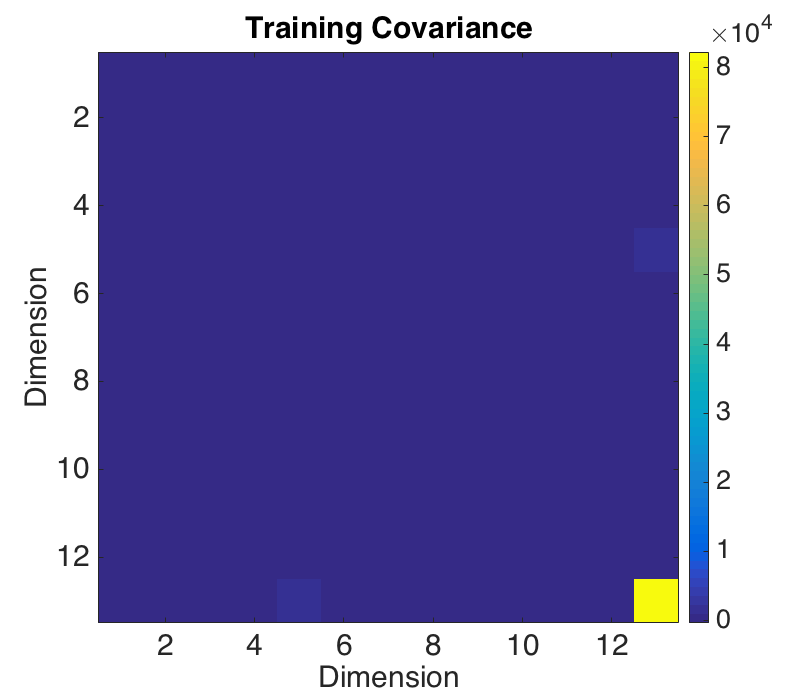
\includegraphics[width=\linewidth]{pic/covtraining.png}
    \caption{Colour map of covariance of training data.}
    \label{fig:covtrainingone}
\end{figure}

This is further seen when looking at the mean values in each dimension for the 4 sets of unmodified data, shown in Table \ref{tbl:trainingmean}. Dimension 13 has the largest magnitude, and this is the cause for the skewed data.

\begin{table}[!ht]
\centering
\caption{Means of Unmodified Data}
\label{tbl:trainingmean}
\begin{tabular}{|r|llll|}
\hline
\textbf{Dimension} & \textbf{All Training} & \textbf{Class 1} & \textbf{Class 2} & \textbf{Class 3} \\ \hline
1 & 12.719 & 13.484 & 11.989 & 12.859\\
2 & 2.262 & 1.959 & 1.846 & 3.242\\
3 & 2.379 & 2.487 & 2.269 & 2.409\\
4 & 19.506 & 17.541 & 20.013 & 21.156\\
5 & 99.542 & 105.000 & 94.106 & 100.875\\
6 & 2.277 & 2.783 & 2.286 & 1.647\\
7 & 2.006 & 2.924 & 2.078 & 0.782\\
8 & 0.357 & 0.291 & 0.358 & 0.438\\
9 & 1.561 & 1.815 & 1.673 & 1.088\\
10 & 4.824 & 5.253 & 2.959 & 7.040\\
11 & 0.959 & 1.059 & 1.073 & 0.668\\
12 & 2.601 & 3.132 & 2.799 & 1.663\\
13 & 737.110 & 1070.385 & 522.213 & 646.562\\ \hline
\end{tabular}
\end{table}

\subsubsection{Normalised Training Data}
The same process is repeated with the normalised data. To save space, once again, the covariance matrices for the different classes can be found in Appendix \ref{sec:covtraining} as Figure \ref{fig:covl2all}, but Figure \ref{fig:covl2one} shows the colour plot for the covariance matrix of all the normalised training data. Along with that, Table \ref{tbl:l2mean} shows the mean values.

\begin{figure}[!ht]
    \centering
    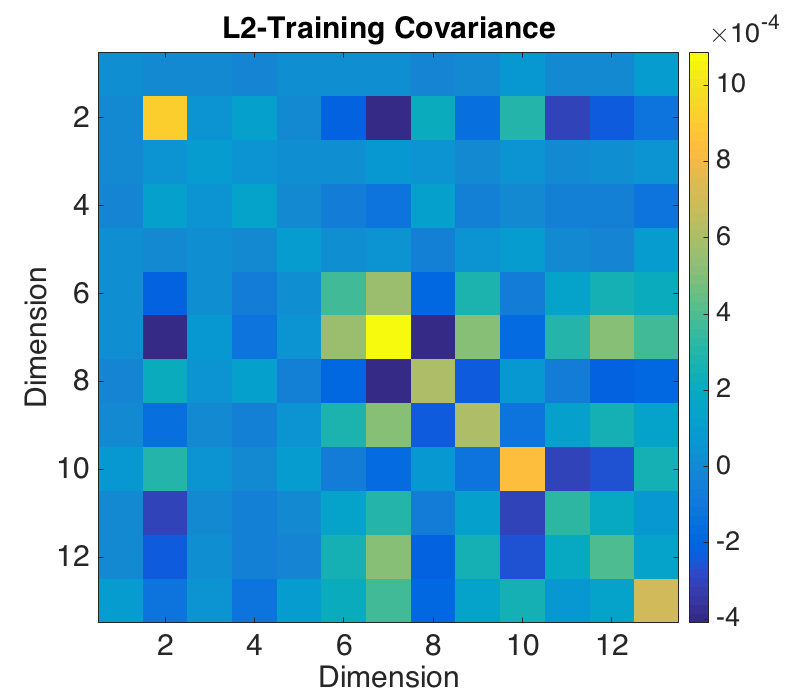
\includegraphics[width=\linewidth]{pic/covl2.png}
    \caption{Colour map of covariance of normalised training data.}
    \label{fig:covl2one}
\end{figure}

\begin{table}[!ht]
\centering
\caption{Means of Normalised Data}
\label{tbl:l2mean}
\begin{tabular}{|r|llll|}
\hline
\textbf{Dimension} & \textbf{All Training} & \textbf{Class 1} & \textbf{Class 2} & \textbf{Class 3} \\ \hline
1 & 0.073 & 0.078 & 0.069 & 0.074\\
2 & 0.066 & 0.057 & 0.053 & 0.094\\
3 & 0.075 & 0.078 & 0.071 & 0.076\\
4 & 0.074 & 0.066 & 0.076 & 0.080\\
5 & 0.074 & 0.078 & 0.070 & 0.075\\
6 & 0.072 & 0.088 & 0.072 & 0.052\\
7 & 0.067 & 0.097 & 0.069 & 0.026\\
8 & 0.070 & 0.057 & 0.070 & 0.086\\
9 & 0.069 & 0.080 & 0.074 & 0.048\\
10 & 0.065 & 0.071 & 0.040 & 0.095\\
11 & 0.073 & 0.081 & 0.082 & 0.051\\
12 & 0.072 & 0.087 & 0.078 & 0.046\\
13 & 0.068 & 0.099 & 0.048 & 0.060\\ \hline
\end{tabular}
\end{table}

The data's means are very much in the same range, which allows the covariances to be in the same range. This means displaying them all as the same scale is possible in the colour map. Knowing that a covariance of zero is a necessary, but not sufficient condition of independence, the dimension pairs that have the lowest covariances are the ones that are the most likely to be independent. 

\subsection{Nearest Neighbour Classification}
Each test data point was assigned a class based on the class of the closest training data point to it. Different measurements were used to represent this concept of ``closeness''. The first one is the L1 distance, or the Manhattan distance. This is expressed with Equation \ref{eq:l1} for 2 $p$-dimensional vectors, $x$ and $y$.
\begin{align}
  L_1 \left( x, y \right) &= \sum_{i = 1}^{p} \lvert x_i  - y_i \rvert \label{eq:l1}
\end{align}
The second is the L2, or Euclidean distance, in Equation \ref{eq:l22}. Equation \ref{eq:chi} shows the Chi-Squared formula, Equation \ref{eq:intersection} shows the histogram intersection formula, and finally Equation \ref{eq:corr} shows the correlation formula. The functions written to implement these metrics can be found in the Appendix.
\begin{align}
  L_2 \left( x, y \right) &= \sum_{i = 1}^{p} \left( x_i  - y_i \right) ^2 \label{eq:l22}\\
  \mathcal{X}^2 \left( x, y \right) &= \frac{1}{2} \sum_{i = 1}^{p} \frac{\left( x_i - y_i \right) ^2 }{\left( x_i + y_i \right)} \label{eq:chi}\\
  \cap \left( x, y \right) &= \sum_{i = 1}^{p} \min \left( x_i, y_i \right) \label{eq:intersection}\\
  CrossCorr &= \sum_{i = 1}^{p} x_i y_i \label{eq:corr}
\end{align}

%-------------------------------------------------------------------------------
% K-means clustering
%-------------------------------------------------------------------------------
\section{K-means clustering}

%-------------------------------------------------------------------------------
% Neural Network
%-------------------------------------------------------------------------------
\section{Neural Network}

% Using Matlab Neural Network toolbox create a network, train and test with the wine data. Vary the parameters of the network to minimize the classification error. Report the observations and compare to the results from Q1 and Q2. Generate another random split of train/test/validation data and repeat the experiment.

Neural networks are an often-used method of pattern recognition, due to their high accuracy, low error rates, and ease of use. They are flexible, and so can be adapted to most pattern recognition problems, such as the use of Convolutional Neural Networks (CNNs) in image recognition, an industry standard.

Neural networks take inspiration from biological neurons, which are interconnected and transmit information using sudden spikes in chemical levels. This is a process that can be simulated in software, including using MATLAB's neural network toolbox (NNT); this toolbox allows the creation, training and testing of various types of neural network. Figures \ref{fig:nnt_perf} and \ref{fig:nnt_vis} show the NNT performance evaluation and visualisation of an example network respectively, with two hidden layers each of 10 neurons in a fitting network configuration.

\begin{figure}[!ht]
    \centering
    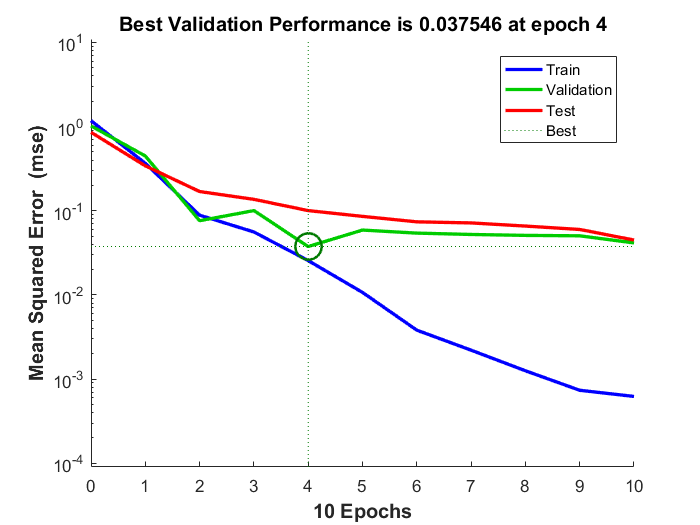
\includegraphics[width=\linewidth]{pic/performance}
    \caption{NNT Performance Evaluation}
    \label{fig:nnt_perf}
\end{figure}

\begin{figure}[!ht]
    \centering
    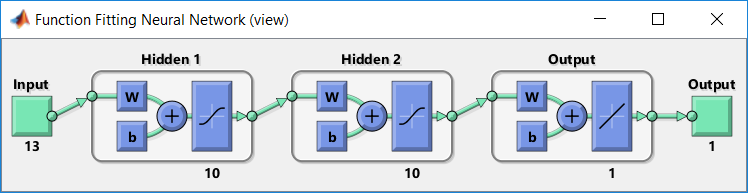
\includegraphics[width=\linewidth]{pic/view_twolayer}
    \caption{NNT Network Visualisation}
    \label{fig:nnt_vis}
\end{figure}

This section tests the use of neural networks to minimise the Mean Squared Error (MSE), as a measure of the performance of the network. First the number of hidden neurons in a single layer fitting network is varied to test performance; results for a standard partition are shown in Table \ref{tbl:unmixed}. The fitting network was used as one of the most flexible types offered by the NNT, and most networks perform with near-optimal results using only a single hidden layer. The code used to generate these results is shown in the Appendix.

The two training algorithms with the minimum mean squared error (MSE) were determined; the results are shown in Figure \ref{fig:unmixed_full}. The effects of overfitting are clearly shown by the huge spike in both algorithms after around 100 hidden neurons. The comparison between the two algorithms is more clearly seen in Figure \ref{fig:unmixed_limited}, which limits the x-axis to 100 hidden neurons.

\begin{figure}[!ht]
    \centering
    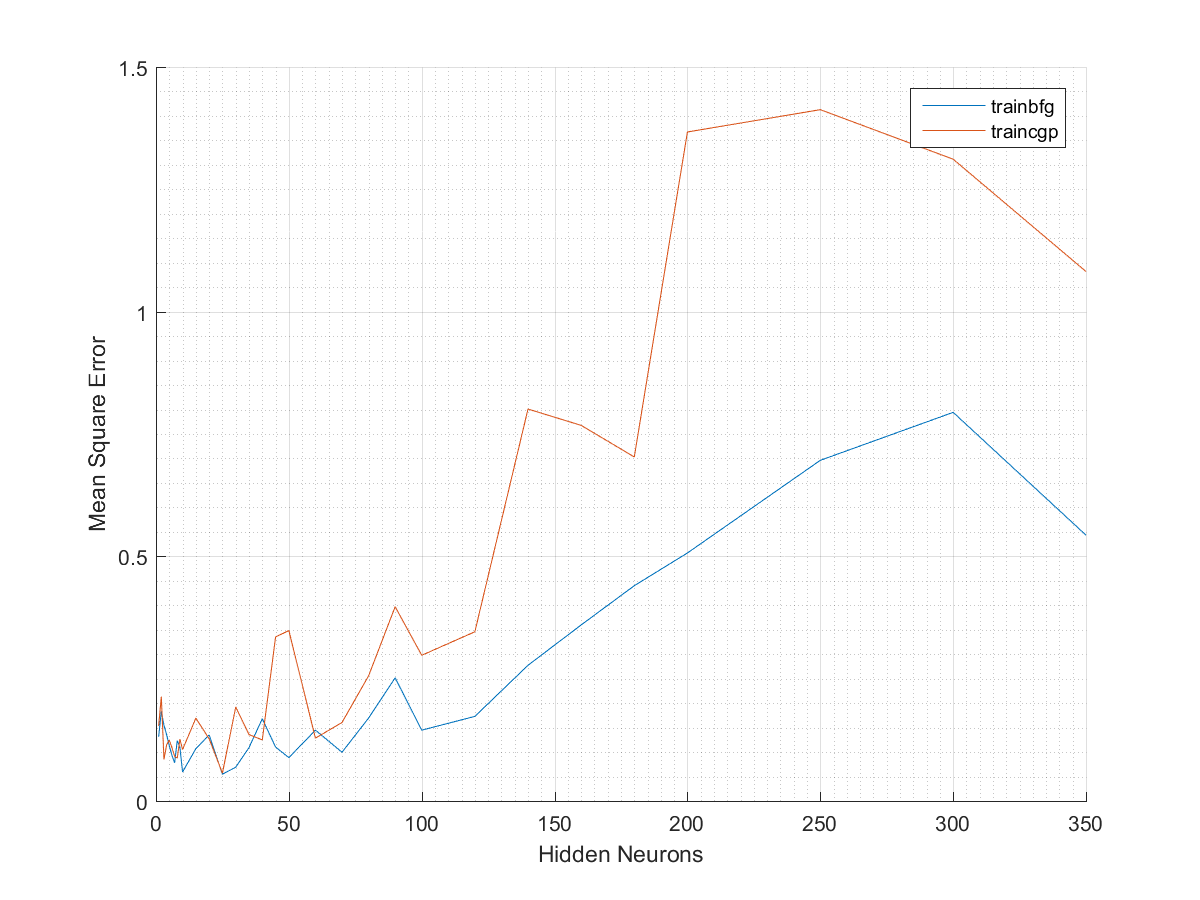
\includegraphics[width=\linewidth]{pic/unmixed_best_fullrange.png}
    \caption{MSE of best performing algorithms}
    \label{fig:unmixed_full}
\end{figure}

\begin{figure}[!ht]
    \centering
    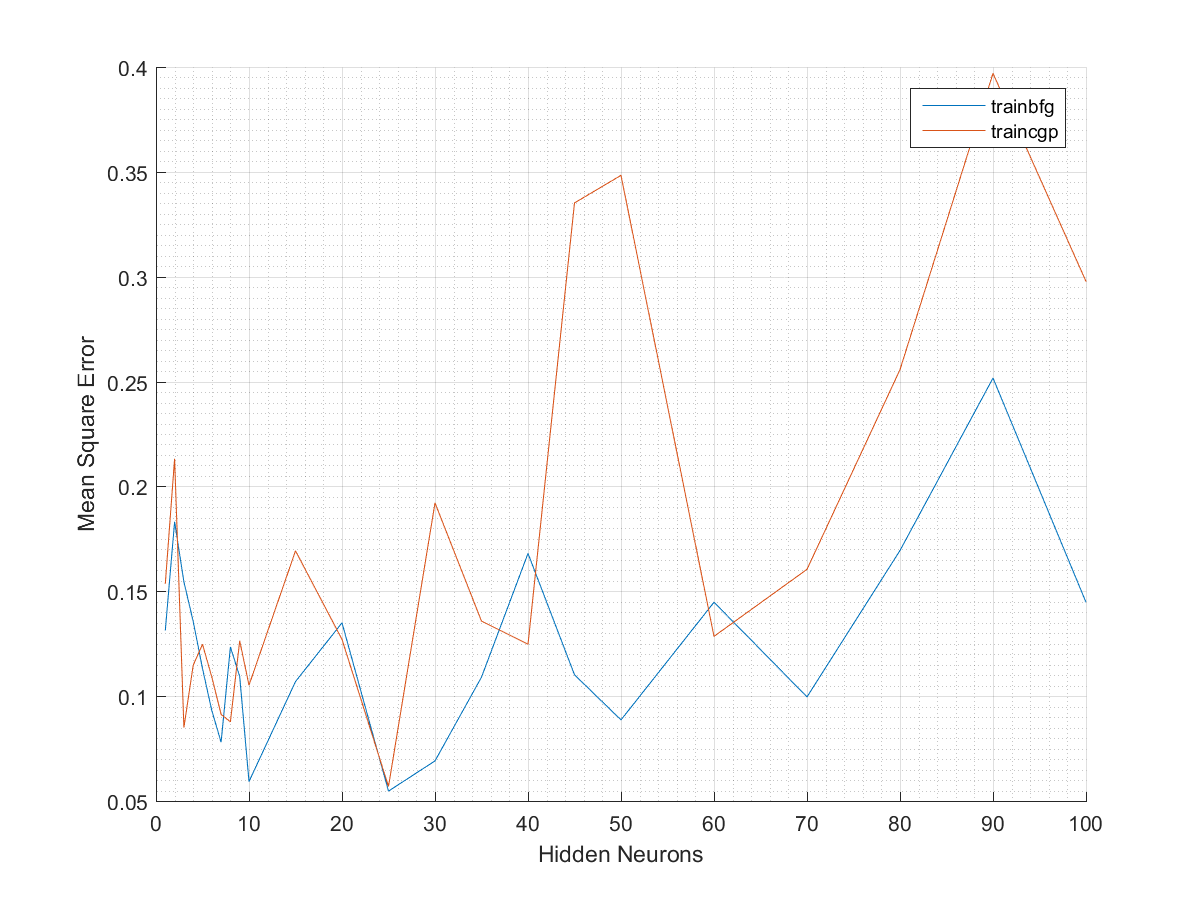
\includegraphics[width=\linewidth]{pic/unmixed_best_limited.png}
    \caption{MSE of best performing algorithms with limited axis}
    \label{fig:unmixed_limited}
\end{figure}

The graphs in the figures show a large variation in MSE between the lower numbers of hidden neurons, but overall there is a downward trend towards the apparent optimum of 25 hidden neurons, which indicates underfitting. After the lowest point, there is an upward trend, which indicates overfitting. Thus, the optimal number of nodes to use is likely between 10 and 50. The best performing algorithm from this data set is the \textit{trainbfg} algorithm.

However, although the standard partition provides an even comparison with other tasks, it does not provide the optimal method of training a network, which is to use a random partition. Therefore, the data in Table \ref{tbl:mixed} show the results of repartitioning with the same ratios, but in a random order. The graph is shown in Figure \ref{fig:mixed_limited}, already limited to 100 neurons due to the same overfitting effect as with the standard partition data.

With randomly partitioned data, the most effective training algorithm is \textit{trainlm} with 15 hidden neurons, but the graph shows that overall \textit{trainbr} is a more effective algorithm, even reducing the effects of overfitting. This is in contrast to the standard partition, which shows other algorithms to be more effective, but more surprisingly the random data shows a lower MSE overall. This implies that using random partitioning is a more effective method of training a neural network than a fixed or contiguous partitioning method; this is further backed up by the first 100\% classification accuracy results. The random partitioning data also shows that the optimum number of hidden neurons to use is between 10 and 50 neurons.

\begin{table}
\centering
\caption{Standard Partition - Hidden Neurons Comparison}
\label{tbl:unmixed}
\begin{tabular}{llllll}
\hline
\textbf{Algorithm} & \textbf{Neurons} & \textbf{Time to Train (s)} & \textbf{Accuracy} & \textbf{MSE} \\ \hline
trainbfg & 15 & 0.15658 & 0.9 & 0.10695 \\ \hline
trainbfg & 20 & 0.23614 & 0.8 & 0.13496 \\ \hline
trainbfg & 25 & 0.82571 & 0.95 & 0.054725 \\ \hline
trainbfg & 30 & 0.76897 & 0.95 & 0.069127 \\ \hline
trainbfg & 35 & 0.70948 & 0.85 & 0.10906 \\ \hline

traincgp & 15 & 0.066146 & 0.825 & 0.16928 \\ \hline
traincgp & 20 & 0.09904 & 0.875 & 0.12706 \\ \hline
traincgp & 25 & 0.10311 & 0.95 & 0.05694 \\ \hline
traincgp & 30 & 0.075015 & 0.85 & 0.19212 \\ \hline
traincgp & 35 & 0.11164 & 0.85 & 0.13576 \\ \hline
\end{tabular}
\end{table}

\begin{figure}[!ht]
    \centering
    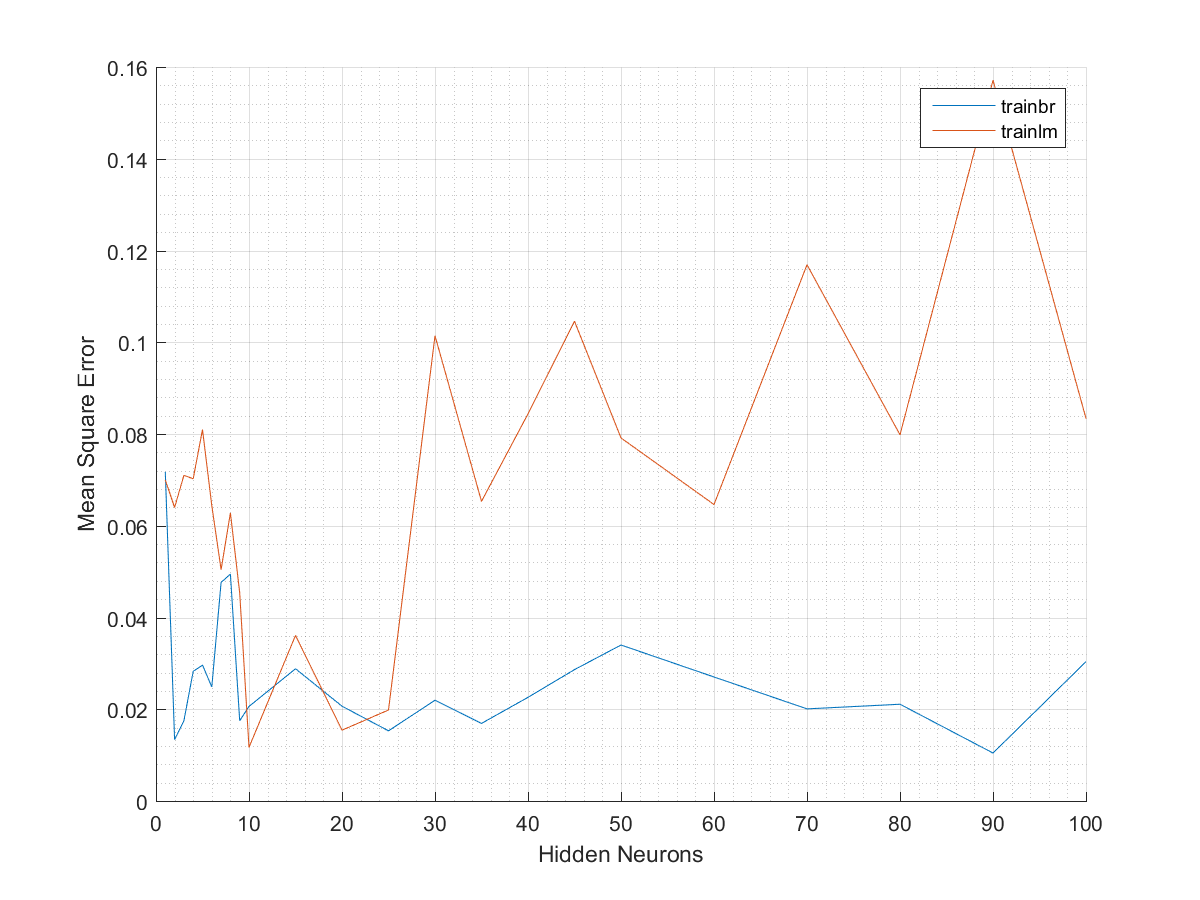
\includegraphics[width=\linewidth]{pic/mixed_best_limited.png}
    \caption{MSE of best performing algorithms with limited axis with random partition}
    \label{fig:mixed_limited}
\end{figure}

\begin{table}
\centering
\caption{Random Partition - Hidden Neurons Comparison}
\label{tbl:mixed}
\begin{tabular}{llllll}
\hline
\textbf{Algorithm} & \textbf{Neurons} & \textbf{Time to Train (s)} & \textbf{Accuracy} & \textbf{MSE} \\ \hline
trainbr & 15 & 5.8827 & 0.975 & 0.028823 \\ \hline
trainbr & 20 & 8.1333 & 0.975 & 0.020667 \\ \hline
trainbr & 25 & 14.6828 & 1 & 0.015294 \\ \hline
trainbr & 30 & 20.2646 & 0.975 & 0.021972 \\ \hline
trainbr & 35 & 28.5412 & 1 & 0.016915 \\ \hline

trainlm & 15 & 0.0657085 & 0.95 & 0.036084 \\ \hline
trainlm & 20 & 0.0607793 & 1 & 0.015435 \\ \hline
trainlm & 25 & 0.0679456 & 1 & 0.019838 \\ \hline
trainlm & 30 & 0.0846978 & 0.85 & 0.10142 \\ \hline
trainlm & 35 & 0.0921787 & 0.975 & 0.065321 \\ \hline
\end{tabular}
\end{table}

% TODO Decide whether to visualise matlab's performance stuff. Should just be in pic folder, but where does it fit?

The examination of neural networks thus far has shown that the most effective number of neurons for a single layer fitting network is in the range of 10-50 approximately. To further minimise the MSE in neural networks, multiple types of network were investigated, simultaneously with the number of layers per network. The code for this may be found in the Appendix; the results with minimum MSE are shown in Tables \ref{tbl:unmixed_networks} and \ref{tbl:mixed_networks}, representing standard and random partition results respectively.

% Tables of interesting data from network and layers comparison
\begin{table}
\centering
\caption{Standard Partition - Network and Layer Comparison}
\label{tbl:unmixed_networks}
\begin{tabular}{llllll}
\hline
\textbf{Network} & \textbf{Algorithm} & \textbf{Layers} & \textbf{Neurons} & \textbf{$T_{train}$} & \textbf{MSE} \\ \hline
pattern & trancgf & 3 & 20 & 0.086992 & 0.034907 \\ \hline
pattern & trainscg & 3 & 20 & 0.065218 & 0.040891 \\ \hline
pattern & trainlm & 2 & 10 & 0.083229 & 0.042546 \\ \hline
pattern & traincgp & 1 & 40 & 0.053625 & 0.0484 \\ \hline
fit & trainbfg & 2 & 30 & 38.0862 & 0.050361 \\ \hline
\end{tabular}
\end{table}

\begin{table}
\centering
\caption{Random Partition - Network and Layer Comparison}
\label{tbl:mixed_networks}
\begin{tabular}{llllll}
\hline
\textbf{Network} & \textbf{Algorithm} & \textbf{Layers} & \textbf{Neurons} & \textbf{$T_{train}$} & \textbf{MSE} \\ \hline
fit & trainbr & 2 & 10 & 6.7953 & 0.01676 \\ \hline
fit & trainbr & 1 & 10 & 0.9048 & 0.01691 \\ \hline
pattern & trainlm & 3 & 25 & 4.2124 & 0.01707 \\ \hline
pattern & trainscg & 3 & 15 & 0.0668& 0.01846 \\ \hline
feedforward & traincgp & 3 & 15 & 0.1105 & 0.01892 \\ \hline
\end{tabular}
\end{table}

The standard partition shows that a different type of network has proved most effective. \textit{Patternnet} is the network that is intended for use in pattern recognition applications, such as this one. However, the MSE of standard partition is still greater than that attained by randomly partitioned data, which uses a fitting network with \textit{trainbr} algorithm as the most effective method, matching very closely with the results of the previous data set. In fact, the previous set of data showed a lower MSE using \textit{trainbr} with a single layer of 25 neurons, which was not investigated in the latter data set due to the large amount of training time required.

Overall, the data shown in this section suggests that the most effective method of minimising error from a neural network is to randomly partition the data, and use a fitting network of a single layer of 25 neurons with the \textit{trainbr} training algorithm. It is possible that more layers of 25 neurons would increase accuracy, but at the cost of training and test time with a minimal decrease in MSE.

% TODO compare MSE and accuracy with other tasks

%-------------------------------------------------------------------------------
% Conclusion
%-------------------------------------------------------------------------------
\section{Conclusion}

A conclusion \cite{pca}.

%-------------------------------------------------------------------------------
% References
%-------------------------------------------------------------------------------
\bibliographystyle{unsrt}
\bibliography{pr_refs}

%-------------------------------------------------------------------------------
% Appendix(ces)
%-------------------------------------------------------------------------------
\onecolumn
\section{Appendix} \label{sec:appendix}

\subsection{All Colour Maps of Covariance Matrices}\label{sec:covtraining}
\begin{figure}[!ht]
  \captionsetup[subfigure]{position=b}
  \centering
    \begin{subfigure}{0.45\textwidth}
      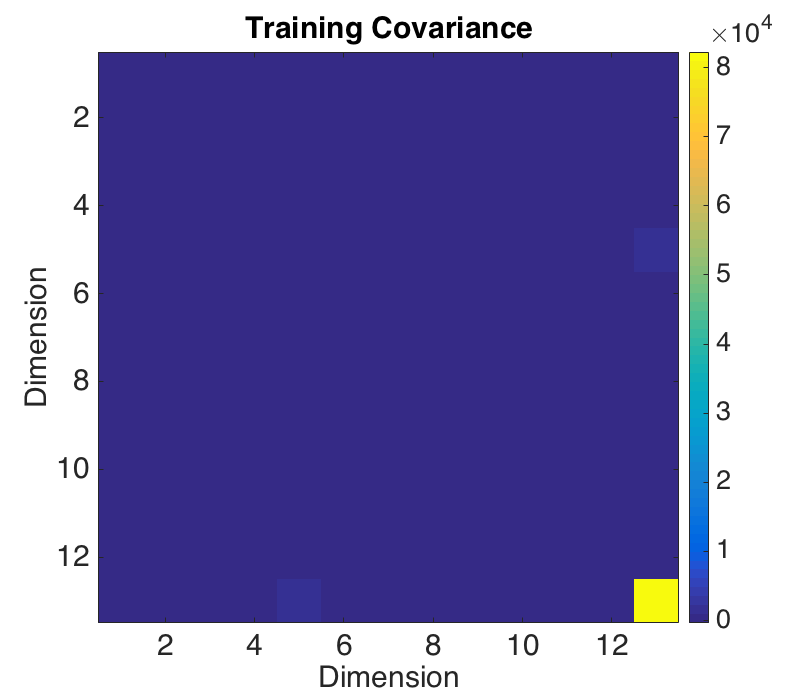
\includegraphics[width=\textwidth]{pic/covtraining.png}
      \caption{Covariance of all.}
      \label{fig:covtraining}
    \end{subfigure}
    ~
    \begin{subfigure}{0.45\textwidth}
      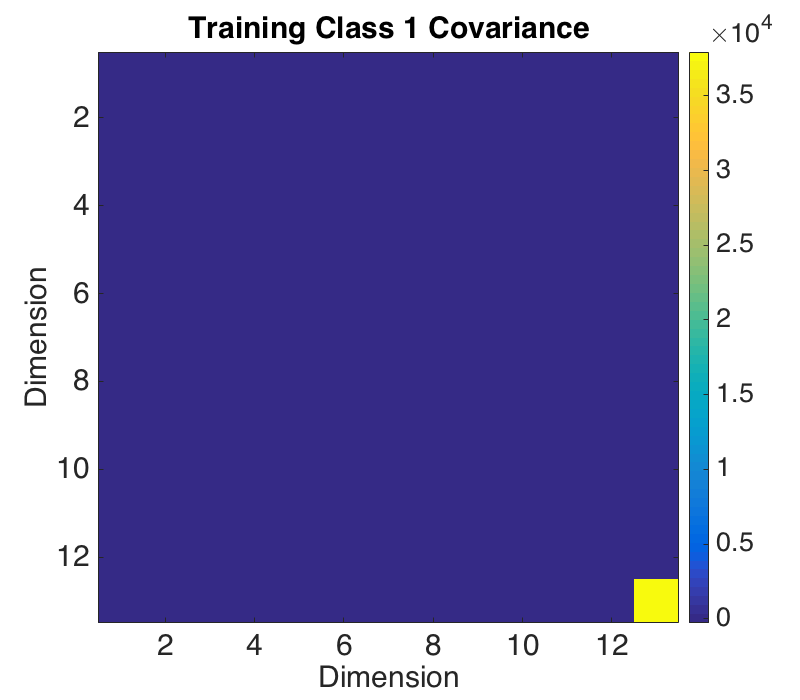
\includegraphics[width=\textwidth]{pic/covclass1.png}
      \caption{Covariance of Class 1.}
      \label{fig:covclass1}
    \end{subfigure}
    \\
    \begin{subfigure}{0.45\textwidth}
      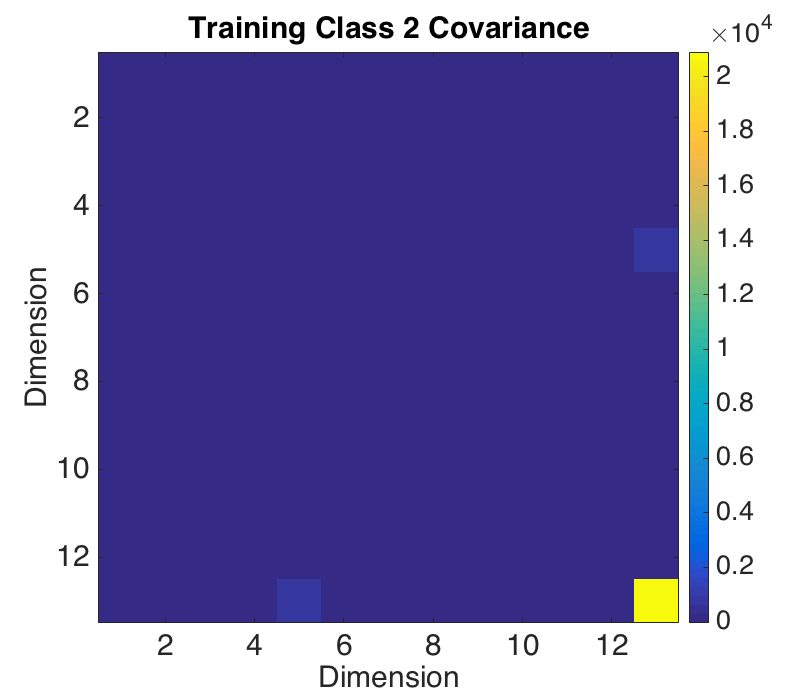
\includegraphics[width=\textwidth]{pic/covclass2.png}
      \caption{Covariance of Class 2.}
      \label{fig:covclass2}
    \end{subfigure}
    ~
    \begin{subfigure}{0.45\textwidth}
      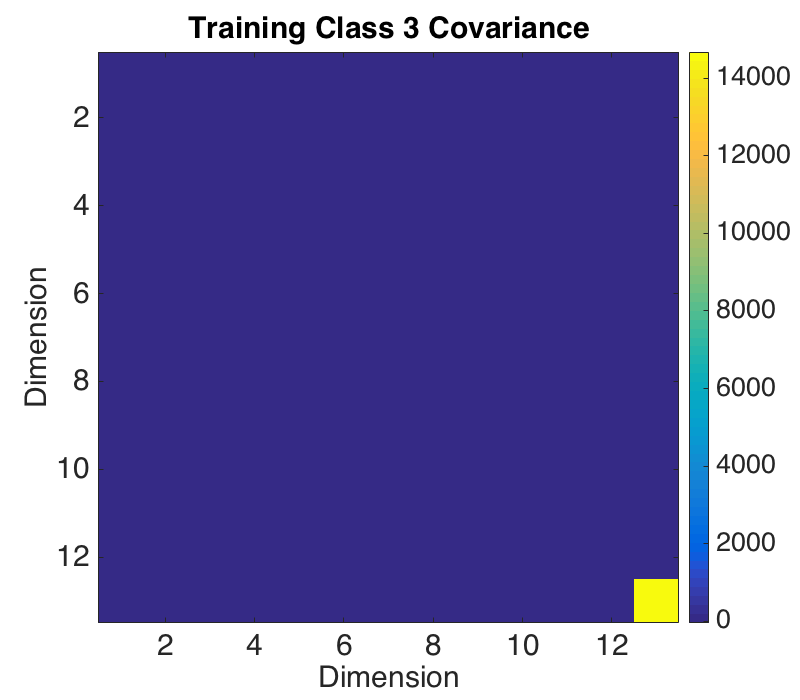
\includegraphics[width=\textwidth]{pic/covclass3.png}
      \caption{Covariance of Class 3.}
      \label{fig:covclass3}
    \end{subfigure}
	\caption{Visualised color maps of covariance matrices from unmodified data.}
  \label{fig:covtrainingall}
\end{figure}
\newpage

\begin{figure}[!ht]
  \captionsetup[subfigure]{position=b}
  \centering
    \begin{subfigure}{0.45\textwidth}
      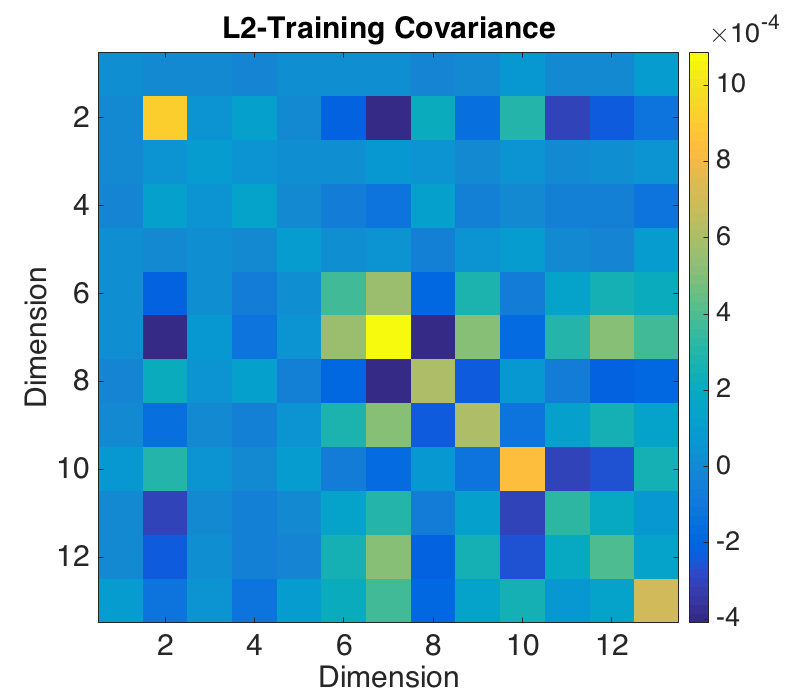
\includegraphics[width=\textwidth]{pic/covl2.png}
      \caption{Covariance of all.}
      \label{fig:covl2}
    \end{subfigure}
    ~
    \begin{subfigure}{0.45\textwidth}
      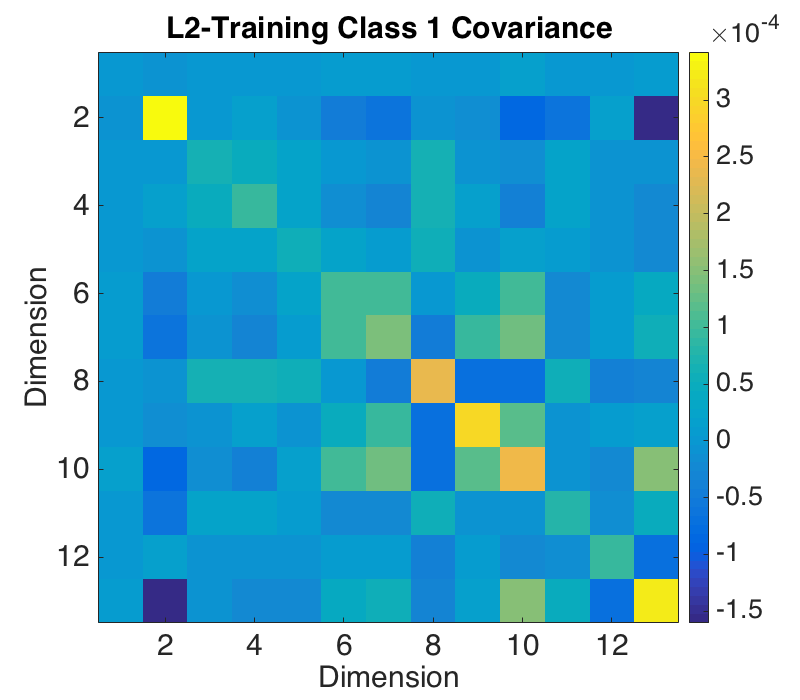
\includegraphics[width=\textwidth]{pic/covl2class1.png}
      \caption{Covariance of Class 1.}
      \label{fig:covl2class1}
    \end{subfigure}
    \\
    \begin{subfigure}{0.45\textwidth}
      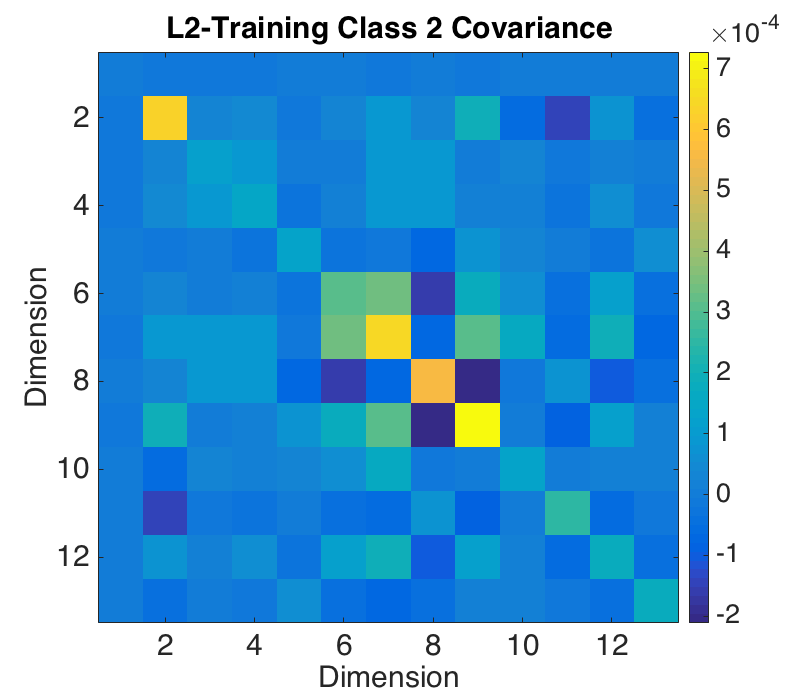
\includegraphics[width=\textwidth]{pic/covl2class2.png}
      \caption{Covariance of Class 2.}
      \label{fig:covl2class2}
    \end{subfigure}
    ~
    \begin{subfigure}{0.45\textwidth}
      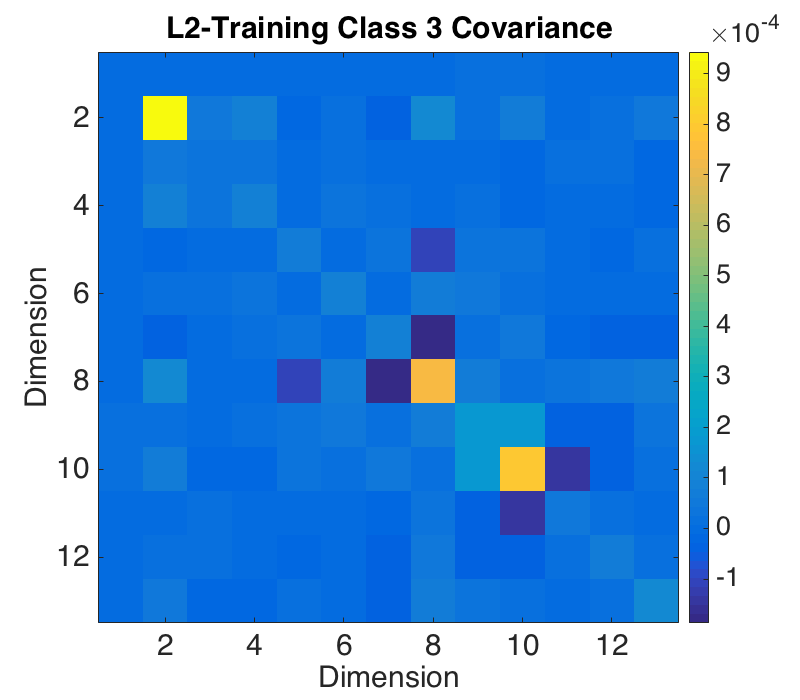
\includegraphics[width=\textwidth]{pic/covl2class3.png}
      \caption{Covariance of Class 3.}
      \label{fig:covl2class3}
    \end{subfigure}
	\caption{Visualised color maps of covariance matrices from L2-normalised data.}
  \label{fig:covl2all}
\end{figure}
\newpage

\subsection{Nearest Neighbour Function Using L1 Metric}
\lstinputlisting[style=Matlab-editor]{src/nearest_neighbour_l1.m}

\subsection{Nearest Neighbour Function Using L2 Metric}
\lstinputlisting[style=Matlab-editor]{src/nearest_neighbour_l2.m}
\newpage

\subsection{Nearest Neighbour Function Using Chi Squared Metric}
\lstinputlisting[style=Matlab-editor]{src/nearest_neighbour_chi.m}

\subsection{Nearest Neighbour Function Using Histogram Intersection Metric}
\lstinputlisting[style=Matlab-editor]{src/nearest_neighbour_intersection.m}
\newpage

\subsection{Nearest Neighbour Function Using Correlation Metric}
\lstinputlisting[style=Matlab-editor]{src/nearest_neighbour_corr.m}

\subsection{Nearest Cluster Function Using \texttt{pdist()}}
\lstinputlisting[style=Matlab-editor]{src/nearest_cluster.m}
\newpage

\subsection{K-Means Clustering Function Using All Four Metrics}
\lstinputlisting[style=Matlab-editor]{src/kmeanmetrics.m}
\newpage

\subsection*{Test set code for Task 3}
\lstinputlisting[style=Matlab-editor]{src/task3_all.m}
\newpage

\subsection*{Making and testing of neural network}
\lstinputlisting[style=Matlab-editor]{src/make_test_nn.m}
\newpage

\subsection*{Test code for various layers/networks for Task 3}
\lstinputlisting[style=Matlab-editor]{src/task3_networks.m}
\newpage

\end{document}
